\chapter{Transfer Matrix Method}

The Transfer Matrix Method (TMM) is a mathematical method for calculating exact solutions to certain statistical mechanical models. The method works by  expressing the partition function in terms of an object called the transfer matrix and the calculation of the exact solution is reduced to  computing its eigenvalues and eigenvectors. The transfer matrix encapsulates the thermodynamic properties of the model through the eigenspectrum of the matrix \cite{Yeomans1992}.

In polymer physics we can use the transfer matrix formalism by treating a polymer as a one-dimensional array of units, much like a one dimensional lattice \cite{Zimm1960,Wartell1985}. Adjacent units make a contribution to the statistical weight of the conformation in a manner that is characterised by the transfer matrix. Since the polymer segments are connected, the state of a given segment depends on the states of the other segments. The partition function of the total system is then given by successive multiplication and summation of all transfer matrices corresponding to the monomer units \cite{Poland1966,Carlon2007}.

The transfer matrix method also has many points in common with a discrete formulation of quantum statistical mechanics, in particular the Feynman formulation in terms of a path integral. Here the transfer matrix method links classical systems described by statistical mechanics in $d$ dimensions with quantum systems in $(d-1)$ dimensions \cite{Parisi1998}.

The transfer matrix method was first introduced into statistical mechanics by Kramers and Wannier \cite{Kramers1941} to find an approximate solution to the statistical mechanics of a two-dimensional ferromagnet, but it was Onsager \cite{Onsager1944} in 1944 who demonstrated its power by calculating the exact partition function of the zero-field version of the Ising model.  The exact solution is covered extensively in the literature \cite{Brush1967, Plischke2006, Yeomans1992, Baxter1982, Newell1953} but for the purpose of understanding the transfer matrix method in its simplest case we begin by introducing the exact solution of the Ising model in one dimension.

\section{One-Dimensional Ising Model}

\begin{figure}[bp]
\centering 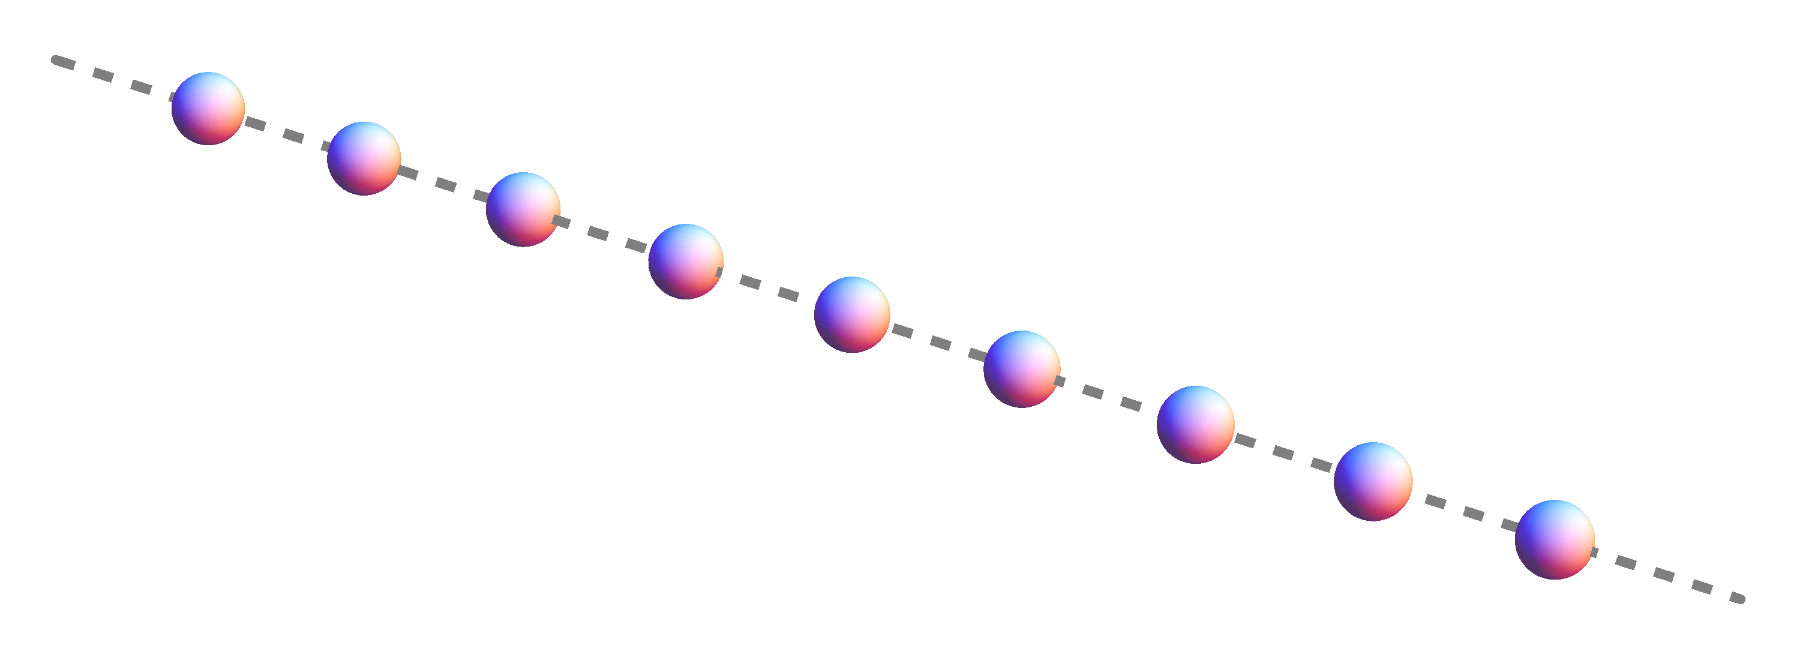
\includegraphics[scale=0.2]{Graphics/TransferMatrix/lattice_1d.png}
\caption{A lattice in one dimension is a set of regularly spaced units.}
\label{fig:1dlattice} 
\end{figure}

The Ising model in one dimension is a classical model for ferromagnetism described by a system of $N$ spins situated regularly on a straight line \figref{1dlattice}.  We denote the value of spin $i$ by $\sigma_i$ which can only take discrete values -1 and 1. In the system we have an external magnetic field interaction of strength $B$, a coupling constant between spin pairs with strength $J$, and the atomic magnetic moment $\mu$. The Hamiltonian for a one-dimensional Ising model is \cite{Newell1953,Yeomans1992}
%
\begin{equation}\label{1disinghamiltonian}
H=-\mu B\sum^{N}_{i=1}\sigma_{i}-J\sum^{N}_{i=1}\sigma_{i}\sigma_{i+1}
\end{equation}
%
where we impose a periodic boundary condition such that 
%
\begin{equation}\label{1disingboundarycondition}
\sigma_{N+1}=\sigma_{1}
\end{equation}
%
This changes the geometry of the straight line lattice into a circle where $\sigma_{N}$ and $\sigma_{1}$ become adjacent neighbours \figref{1dlatticeclosed}. In the Hamiltonian this allows the last term in the sum of interactions to become $\sigma_{N}\sigma_{1}$. Inserting the Hamiltonian into the partition function we get 
%
%The choice of boundary conditions becomes irrelevant in the thermodynamic limit \cite{Yeomans1992}
%
\begin{align}
Z &=\sum\exp\left( -\beta H\right)\\
&=\sum_{\{\sigma_{i}=\pm1\}}\exp\left(\beta\mu B\sum^{N}_{i=1}\sigma_{i}+\beta J\sum^{N}_{i=1}\sigma_{i}\sigma_{i+1}\right)\\
&=\sum_{\{\sigma_{i}=\pm1\}}\prod^{N}_{i=1}\exp\left( \beta \mu B\sigma_{i}\right)\exp\left(\beta J\sigma_{i}\sigma_{i+1}\right) \label{1dising1}
\end{align}
%
\begin{figure}[bp]
\centering 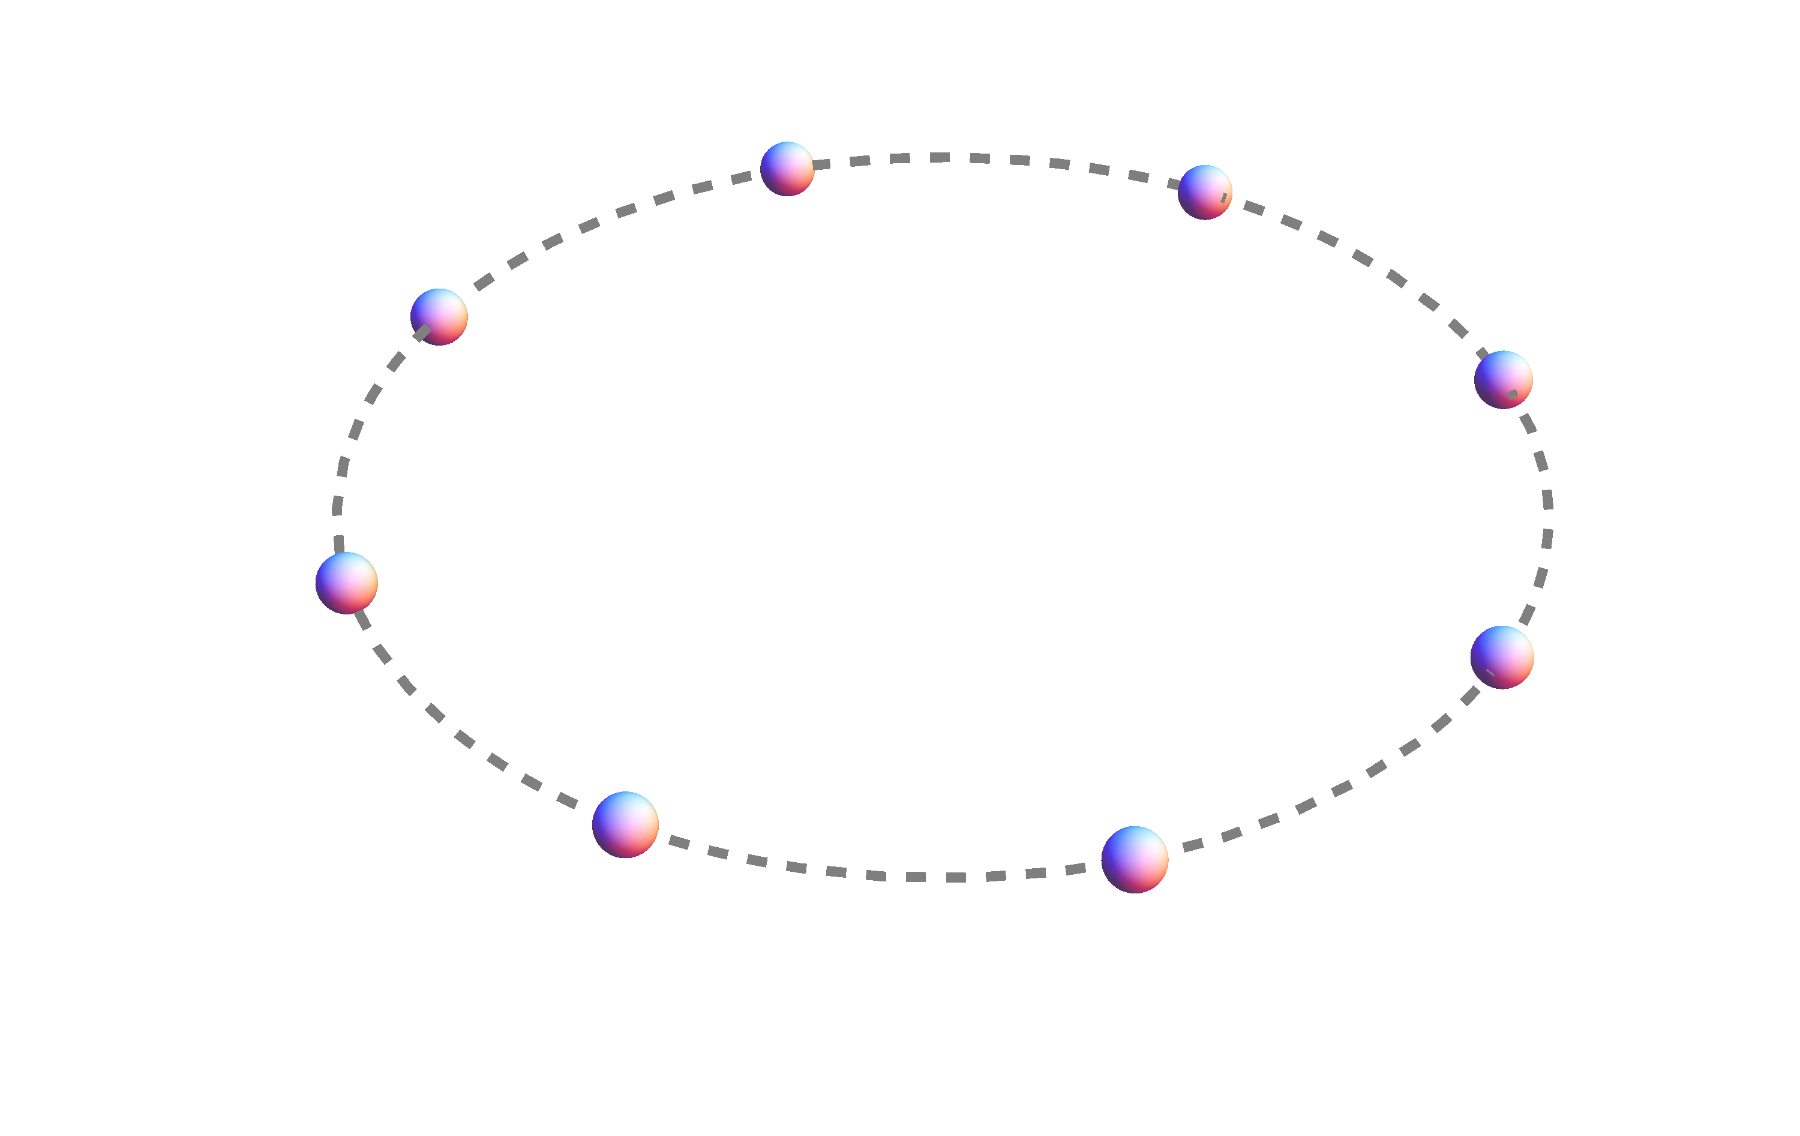
\includegraphics[scale=0.2]{Graphics/TransferMatrix/lattice_1d_closed.png}
\caption{A lattice in one dimension with periodic boundary conditions forms a circle.}
\label{fig:1dlatticeclosed} 
\end{figure}
%
The product of contributions from each spin in the exponential allows us to group adjacent spins together. If we do  this \eqref{1dising1} becomes \cite{Yeomans1992}
%
\begin{align}\label{1disingbeforematrixform}
Z&=\sum_{\{\sigma_{i}=\pm1\}}\exp\left(\beta J\sigma_{1}\sigma_{2}+\frac{\beta B\left(\sigma_{1}+\sigma_{2}\right)}{2}\right)\exp\left(\beta J\sigma_{2}\sigma_{3}+\frac{\beta B\left(\sigma_{2}+\sigma_{3}\right)}{2}\right)...\\
&...\exp\left(\beta J\sigma_{N-1}\sigma_{N}+\frac{\beta B\left(\sigma_{N-1}+\sigma_{N}\right)}{2}\right)\exp\left(\beta J\sigma_{N}\sigma_{1}+\frac{\beta B\left(\sigma_{N}+\sigma_{1}\right)}{2}\right)\nonumber
\end{align}
%
Next we introduce $T\left(\sigma_{i},\sigma_{i+1}\right)$,  which are the elements of a transfer matrix $T$. The rows are labelled by the values of $\sigma_{i}$ and columns by the values $\sigma_{i+1}$.
%
\begin{equation}\label{1disingtransfermatrix}
T\left(\sigma_{i},\sigma_{i+1}\right)=\exp\left(\beta J\sigma_{i}\sigma_{i+1}+\frac{\beta B\left(\sigma_{i}+\sigma_{i+1}\right)}{2}\right)
\end{equation}
%
If we write out the transfer matrix explicitly we get a $2 \times 2$ matrix
%
\begin{equation}
\bordermatrix{&\sigma_{i}=1&\sigma_{i+1}=-1 \cr
\sigma_{i}=1 & \exp\left(\beta J+B\right) & \exp\left(-\beta J \right) \cr
\sigma_{i+1}=-1 & \exp\left(-\beta J \right) & \exp\left(\beta J-B\right) \cr }
\end{equation}
%
Substituting \eqref{1disingtransfermatrix} into \eqref{1disingbeforematrixform}, the transfer matrix allows us to express the partition function  as a product of matrices \cite{Yeomans1992}
%
\begin{equation}
Z=\sum_{\{\sigma_{i}=\pm1\}}T\left(\sigma_{1},\sigma_{2}\right)T\left(\sigma_{2},\sigma_{3}\right)...T\left(\sigma_{N-1},\sigma_{N}\right)T\left(\sigma_{N},\sigma_{1}\right)=\mbox{tr}\left( T^{N}\right)
\end{equation}
%
This equation reduces the calculation of the partition function to the calculation of the trace of an unknown matrix $T^{N}$ . We know from linear algebra that the trace is invariant under cyclic permutations, and therefore using this property in conjunction with an appropriate unitary matrix $U$ and its inverse $U^{-1}$ we can convert the transfer matrix into a diagonal form
%
\begin{equation}
U^{-1}TU= \Lambda =\begin{pmatrix}
\lambda_1 & 0 \\ 
0 & \lambda_2 
\end{pmatrix}
\end{equation}
%
Where $\lambda_1$ and $\lambda_2$ are the eigenvalues of the transfer matrix $T$. Inserting this into the partition function we get
%
\begin{equation}
Z=\mbox{tr}\left(T^{N}\right) = \mbox{tr}\left(\Lambda^{N}\right) = \lambda_1^{N} + \lambda_2^{N}
\end{equation}
%
The eigenvalues of the transfer matrix can be calculated using the eigenvalue equation without explicitly knowing the form of the corresponding eigenvectors
%
\begin{equation}
\det \left| T-\lambda_{i}I\right| =
\begin{vmatrix}
\exp\left(\beta J+\beta B\right)-\lambda_1 & \exp\left(-\beta J \right) \\ \exp\left(-\beta J \right) & \exp\left(\beta J-\beta B\right)-\lambda_2 
\end{vmatrix}=0
\end{equation}
%
where the eigenvalues are \cite{Plischke2006,Yeomans1992}
%
\begin{equation}
\lambda_{1,2}=\exp\left( \beta J \right)\cosh \beta B\pm\sqrt{ \exp\left(2 \beta J\right)\sinh^{2}\beta B + \exp\left(-2\beta J\right)}
\end{equation}
%
The analysis using the transfer matrix gives surprising results in the thermodynamic limit $N \to \infty$ where the boundary effects become negligible only the largest eigenvalue is relevant. In the thermodynamic limit the free energy per spin is given by
%
\begin{align}
F&=-k_{B}T\lim_{N\to\infty}\frac{1}{N}\ln Z_{N}\\
&=-k_{B}T\lim_{N\to\infty}\frac{1}{N}\ln  \left\{ \lambda_{1}^{N}+\lambda_{2}^{N}\right\} \label{fe_2b2}
\end{align}
%
For the more general case where the transfer matrix is larger than a $2 \times 2$ matrix the set of eigenvalues go beyond $\lambda_{1}$ and $\lambda_{2}$, and \eqref{fe_2b2} becomes  
%
\begin{equation}
F=-k_{B}T\lim_{x\to\infty}\frac{1}{N}\ln \left\{ \lambda_{1}^{N}\left(1+\sum_{i}\frac{\lambda_{i}^{N}}{\lambda_{1}^{N}} \right)\right\} \label{fe_general}
\end{equation}
%
With $\lambda_{1}$ being the largest eigenvalue. Since the ratio $\lambda_{i}/\lambda_{1}$ is always less than unity, taking $N\to\infty$ leads to $\left(\lambda_{i}/\lambda_{1}\right)^{N}\to 0$ and hence
%
\begin{equation}
F=-k_{B} T \ln\lambda_{1}
\end{equation}
%
This elegantly shows that thermodynamic quantities in the thermodynamic limit $N\to\infty$ depend only on the largest eigenvalue of the transfer matrix, which is often easier to calculate than the entire spectrum of the matrix. Since this is also true for other interacting many-particle systems treated with the transfer matrix method the problem of finding the exact solution within the transfer-matrix approach is reduced to finding the largest eigenvalue. 

\section{Two-Dimensional Ising Model}

For a two dimensional model we consider a spin-$\frac{1}{2}$ Ising model on a square lattice in a vanishing external field. The lattice is defined by $R$ rows and $C$ columns and the Hamiltonian can be written as \cite{Schultz1964}
%
\begin{equation}
H=-J\left(\sum_{i=1}^{R}\sum_{j=1}^{C}\sigma_{i,j}\sigma_{i+1,j}+\sum_{i=1}^{R}\sum_{j=1}^{C}\sigma_{i,j+1}\sigma_{i,j}\right) 
\end{equation}

\begin{figure}[htp]
\centering 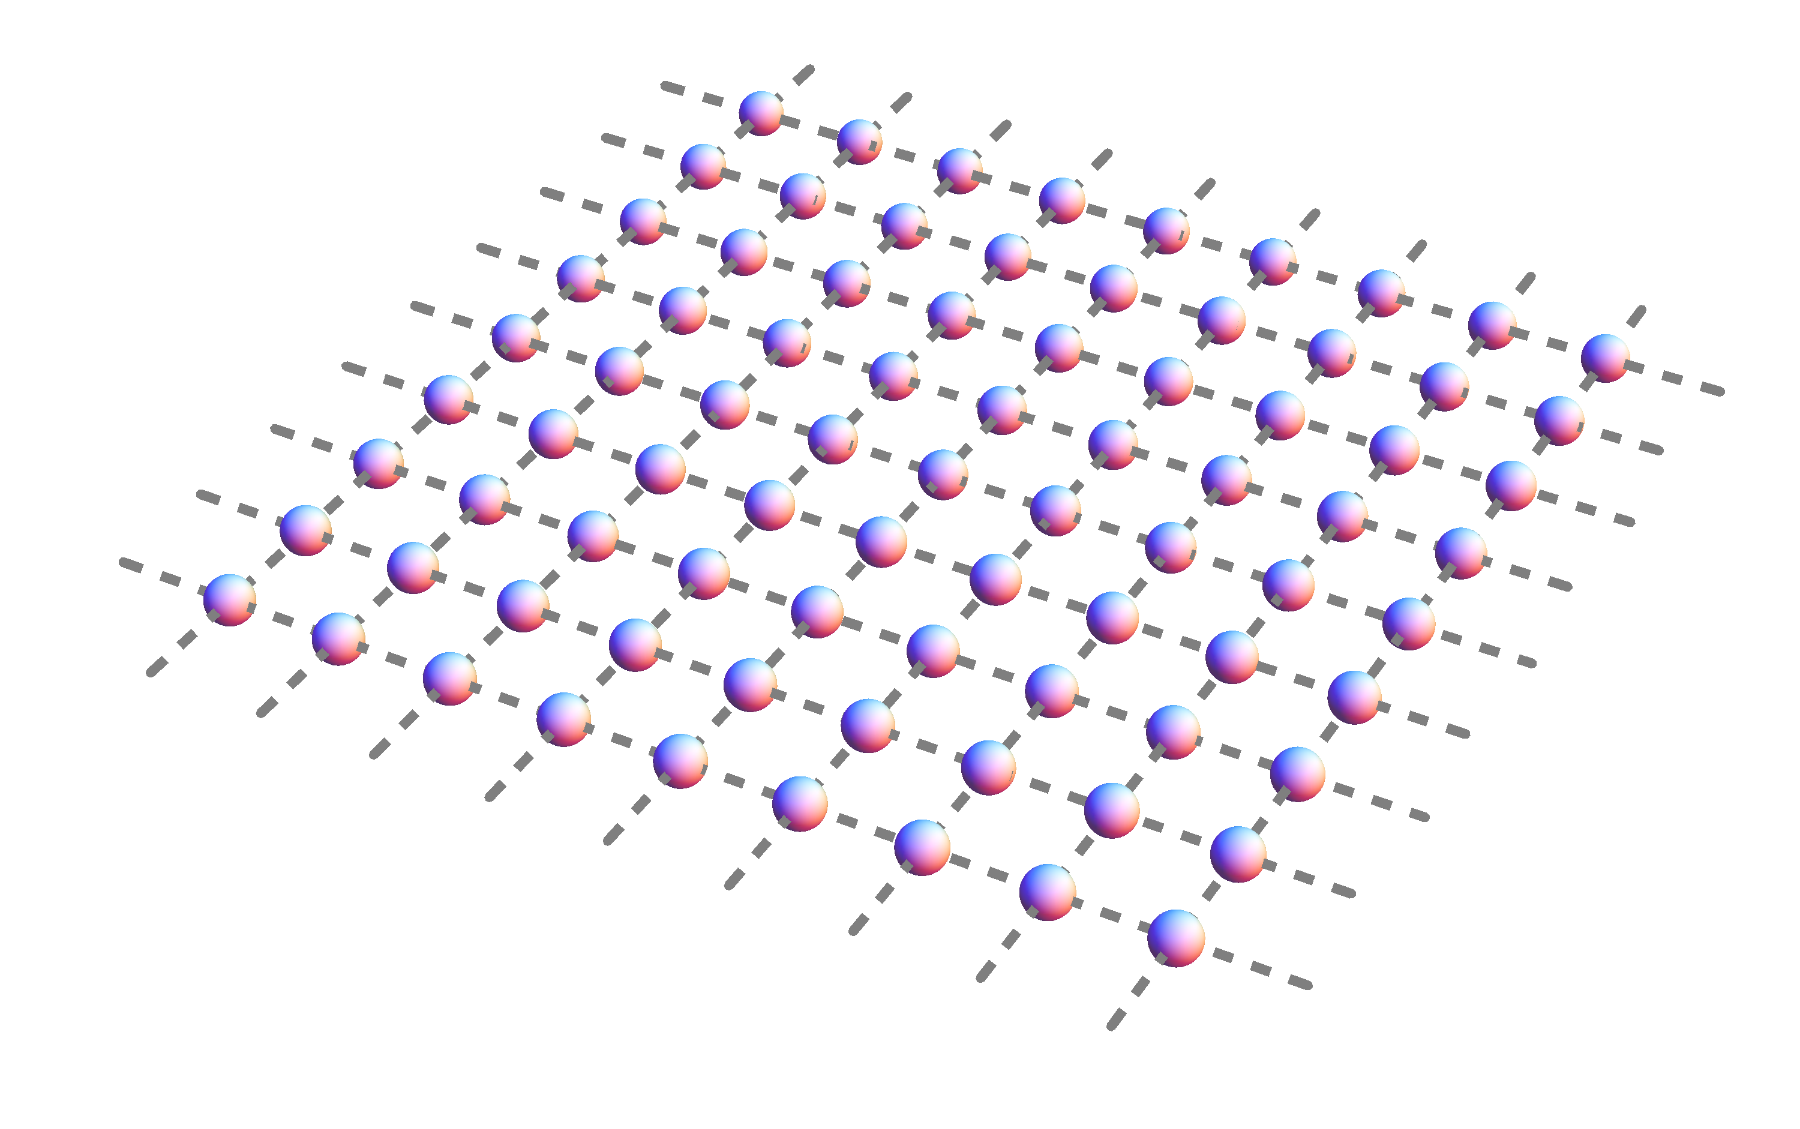
\includegraphics[scale=0.2]{Graphics/TransferMatrix/lattice_2d.png}
\caption{A lattice in two dimensions.}
\label{fig:2dlattice} 
\end{figure}
%
The summations contain two spin coupling interactions between nearest-neighbours: one is for adjacent rows of the square lattice, while the other takes into account adjacent columns. Again, we impose boundary conditions such that the square lattice is continuous
%
\begin{align}
\label{2disingboundarycondition1}
\sigma_{R+1,j}&=\sigma_{1,j}\quad \text{where $j=1,2,3,...,C$}\\
\label{2disingboundarycondition2}
\sigma_{i,C+1}&=\sigma_{i,1}\quad \text{where $i=1,2,3,...,R$}
\end{align}
%
The periodicity of the square lattice makes it topologically equivalent to a 2-torus where the $C^{th}$ column is coupled to the first column, and the  $R^{th}$ row is coupled to the first row. 
%
\begin{figure}[htp]
\centering 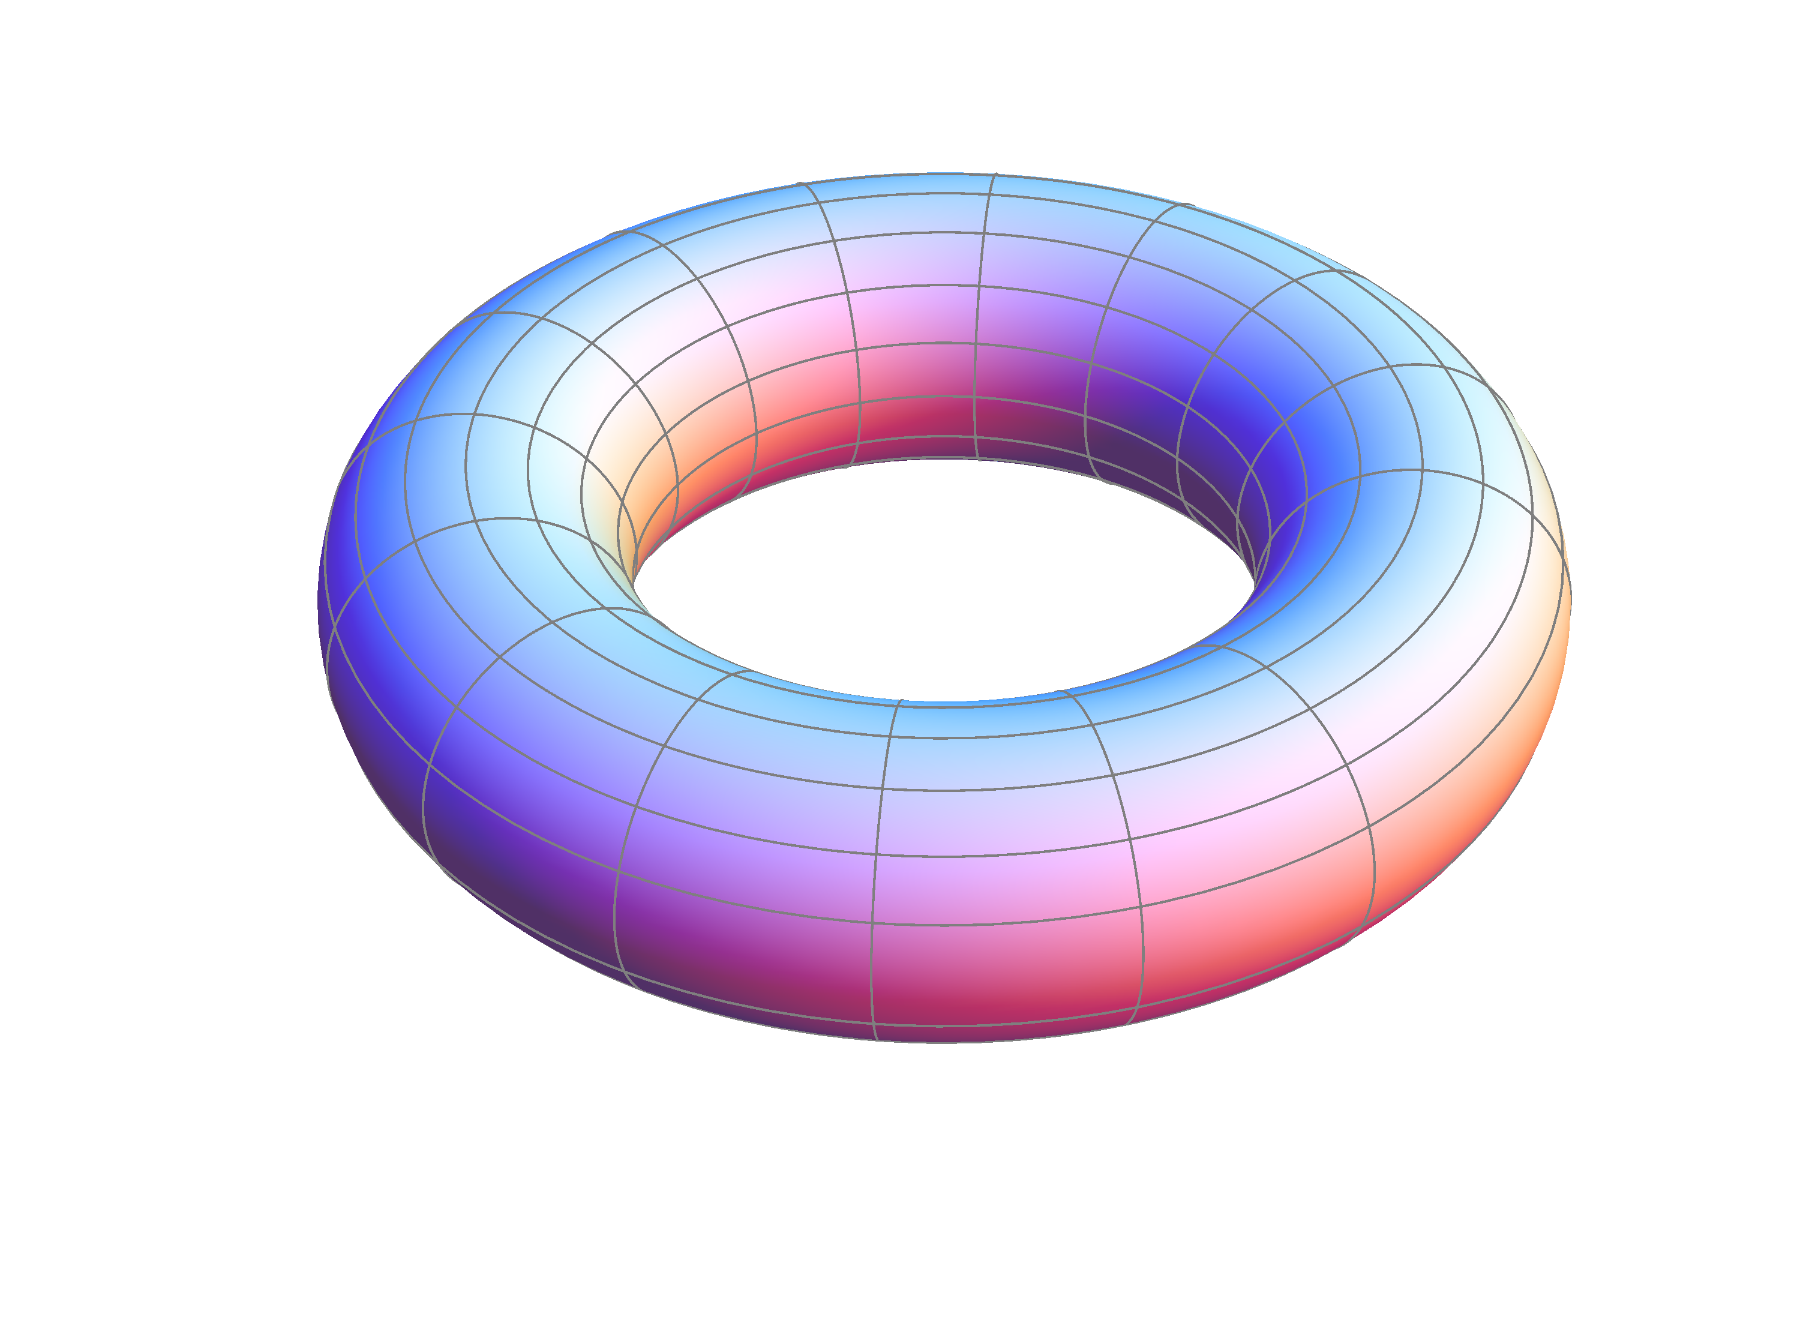
\includegraphics[scale=0.25]{Graphics/TransferMatrix/torus.png}
\caption{The boundary conditions in the vertical and horizontal directions wraps the square lattice into a 2-torus.}
\label{fig:torus} 
\end{figure}
%
We then set the the overall spin configuration of the $j^{th}$ column of spins by a new variable $\xi_{j}$ which has $2^{R}$ possible spin configurations.
%
\begin{equation}
\xi_{j}=\left(\sigma_{1,j},\sigma_{2,j},\sigma_{3,j},\sigma_{4,j},.....,\sigma_{R,j}\right)
\end{equation}
%
The Hamiltonian can then be written as a sum of the interaction energy of individual columns, $H_{1}$, and the interaction energy between adjacent columns, $H_{2}$.
%
\begin{align}
H_{1}\left(\xi_{j}\right)&=-J\sum_{i=1}^{R}\sigma_{i,j}\sigma_{i+1,j}\\
H_{2}\left(\xi_{j},\xi_{j+1}\right)&=-J\sum_{i=1}^{R}\sigma_{i,j}\sigma_{i,j+1}
\end{align}
%
The total Hamiltonian is simply
%
\begin{equation}
H\left(\xi\right)=\sum^{C}_{j=1}H_{1}\left(\xi_{j}\right) + H_{2}\left(\xi_{j},\xi_{j+1} \right)
\end{equation}
%
In the symmetric form the Hamiltonian is
%
\begin{equation}
H\left(\xi\right)= \sum^{C}_{j=1}\frac{1}{2} H_{1} \left(\xi_{j}\right) +\frac{1}{2} H_{1}\left( \xi_{j+1}\right) +  H_{2}\left(\xi_{j},\xi_{j+1} \right)
\end{equation}
%
Inserting this into the partition function  we get the relation
%
\begin{align}
Z&=\sum_{\xi_1}\sum_{\xi_2}\sum_{\xi_3}...\sum_{\xi_C}\exp\left(\sum^{C}_{j=1}-\frac{\beta}{2}\left( H_{1}\left(\xi_{j}\right) +H_{1}\left( \xi_{j+1}\right)\right) -  \beta H_{2}\left(\xi_{j},\xi_{j+1} \right) \right)\nonumber\\
&=\sum_{\xi_1}\sum_{\xi_2}\sum_{\xi_3}...\sum_{\xi_C}\prod_{j=1}^{C}\exp\left( -\frac{\beta}{2}\left( H_{1}\left(\xi_{j}\right) + H_{1}\left(\xi_{j+1}\right)\right) -  \beta H_{2}\left(\xi_{j},\xi_{j+1} \right) \right)
\end{align}
%
which evidently demonstrates the transfer matrix for the 2D Ising model to be
%
\begin{align}
T\left(\xi_j,\xi_{j+1}\right)&= \exp\left( -\frac{\beta}{2}\left( H_{1}\left(\xi_{j}\right) + H_{1}\left(\xi_{j+1}\right)\right) -  \beta H_{2}\left(\xi_{j},\xi_{j+1} \right) \right) \nonumber\\
&=\exp\left( \frac{\beta J}{2}\left( \sum_{i=1}^{R}\sigma_{i,j}\sigma_{i+1,j}   +   \sum_{i=1}^{R}\sigma_{i,j+1}\sigma_{i+1,j+1} \right) + \beta J\sum^{R}_{i=1}\sigma_{i,j}\sigma_{i,j+1} \right)
\end{align}
%
Using these transfer matrices in the partition function we get
%
\begin{equation}
Z=\sum_{\xi_1}\sum_{\xi_2}...\sum_{\xi_C}T\left(\xi_1,\xi_2\right)T\left(\xi_2,\xi_3\right)...T\left(\xi_{C-1},\xi_C\right)T\left(\xi_C,\xi_{1}\right) \label{tm_torus}
\end{equation}
%
At this point we introduce a Kronecker delta defined by the boundary conditions $\delta_{\xi_{C+1},\xi_{1} }$ and then apply the completeness relation to express the delta function as set of eigenfunctions, $\psi_{\mu}$, of the transfer matrix $T\left(\xi_i,\xi_{i+1}\right)$.
%
\begin{equation}
\delta_{\xi_{C+1},\xi_{1} }=\sum_{\mu}\psi_{\mu}^{*}\left(\xi_{1} \right)\psi_{\mu}\left(\xi_{C+1}\right)
\end{equation}
%
The eigenvalue equation is
%
\begin{equation}\label{2devalequation}
\sum_{\xi_{i}}T\left(\xi_i,\xi_{i+1}\right)\psi_{\mu}\left(\xi_{i}\right) = \lambda_{\mu}\psi_{\mu}\left(\xi_{i+1}\right)
\end{equation}
%
The partition function with the complete set of eigenfunctions becomes
%
\begin{equation}
Z=\sum_{\mu}\sum_{\xi_1}\sum_{\xi_2}...\sum_{\xi_C}\sum_{\xi_{C+1}}\psi_{\mu}^{*}\left(\xi_{1} \right)T\left(\xi_1,\xi_2\right)T\left(\xi_2,\xi_3\right)...T\left(\xi_{C-1},\xi_C\right)T\left(\xi_C,\xi_{C+1}\right)\psi_{\mu}\left(\xi_{C+1}\right)\\
\end{equation}
%
Now we use equation \eqref{2devalequation} to contract each transfer matrix in the sum with an appropriate eigenfunction, leaving behind an eigenvalue which is a scalar quantity. We get
%
\begin{equation}
Z=\mbox{tr}\left(T^{C}\right)=\sum_{j=1}^{2^{R}} \lambda_{j}^{C}
\end{equation}
%
In the thermodynamic limit the free energy per spring for a 2D Ising model becomes
%
\begin{align}
F&=-k_{B}T\lim_{R\to\infty}\lim_{C\to\infty}\left\{\frac{1}{RC}\ln \left(\lambda^{C}_{1} + \lambda^{C}_{2} + ... + \lambda^{C}_{2^{R}}\right)\right\} \\
&= -k_{B}T\lim_{R\to\infty}\frac{1}{R}\ln\lambda_{1} - k_{B}T\lim_{R\to\infty}\lim_{C\to\infty}\frac{1}{RC}\ln\left[1+\sum_{i}^{2^R}\left(\frac{\lambda_{g}}{\lambda_{1}}\right)^{C}\right]\\
&= -k_{B}T\lim_{R\to\infty}\frac{1}{R} \ln \lambda_{1}
\end{align}
%
The calculation of the largest eigenvalue of the $T\left(\xi_i,\xi_{i+1}\right)$ matrix goes beyond the scope of this thesis but here again we have clearly demonstrated the use of the transfer matrix method in finding the exact solution to the 2D Ising model.
%
\begin{figure}[bp]
\centering 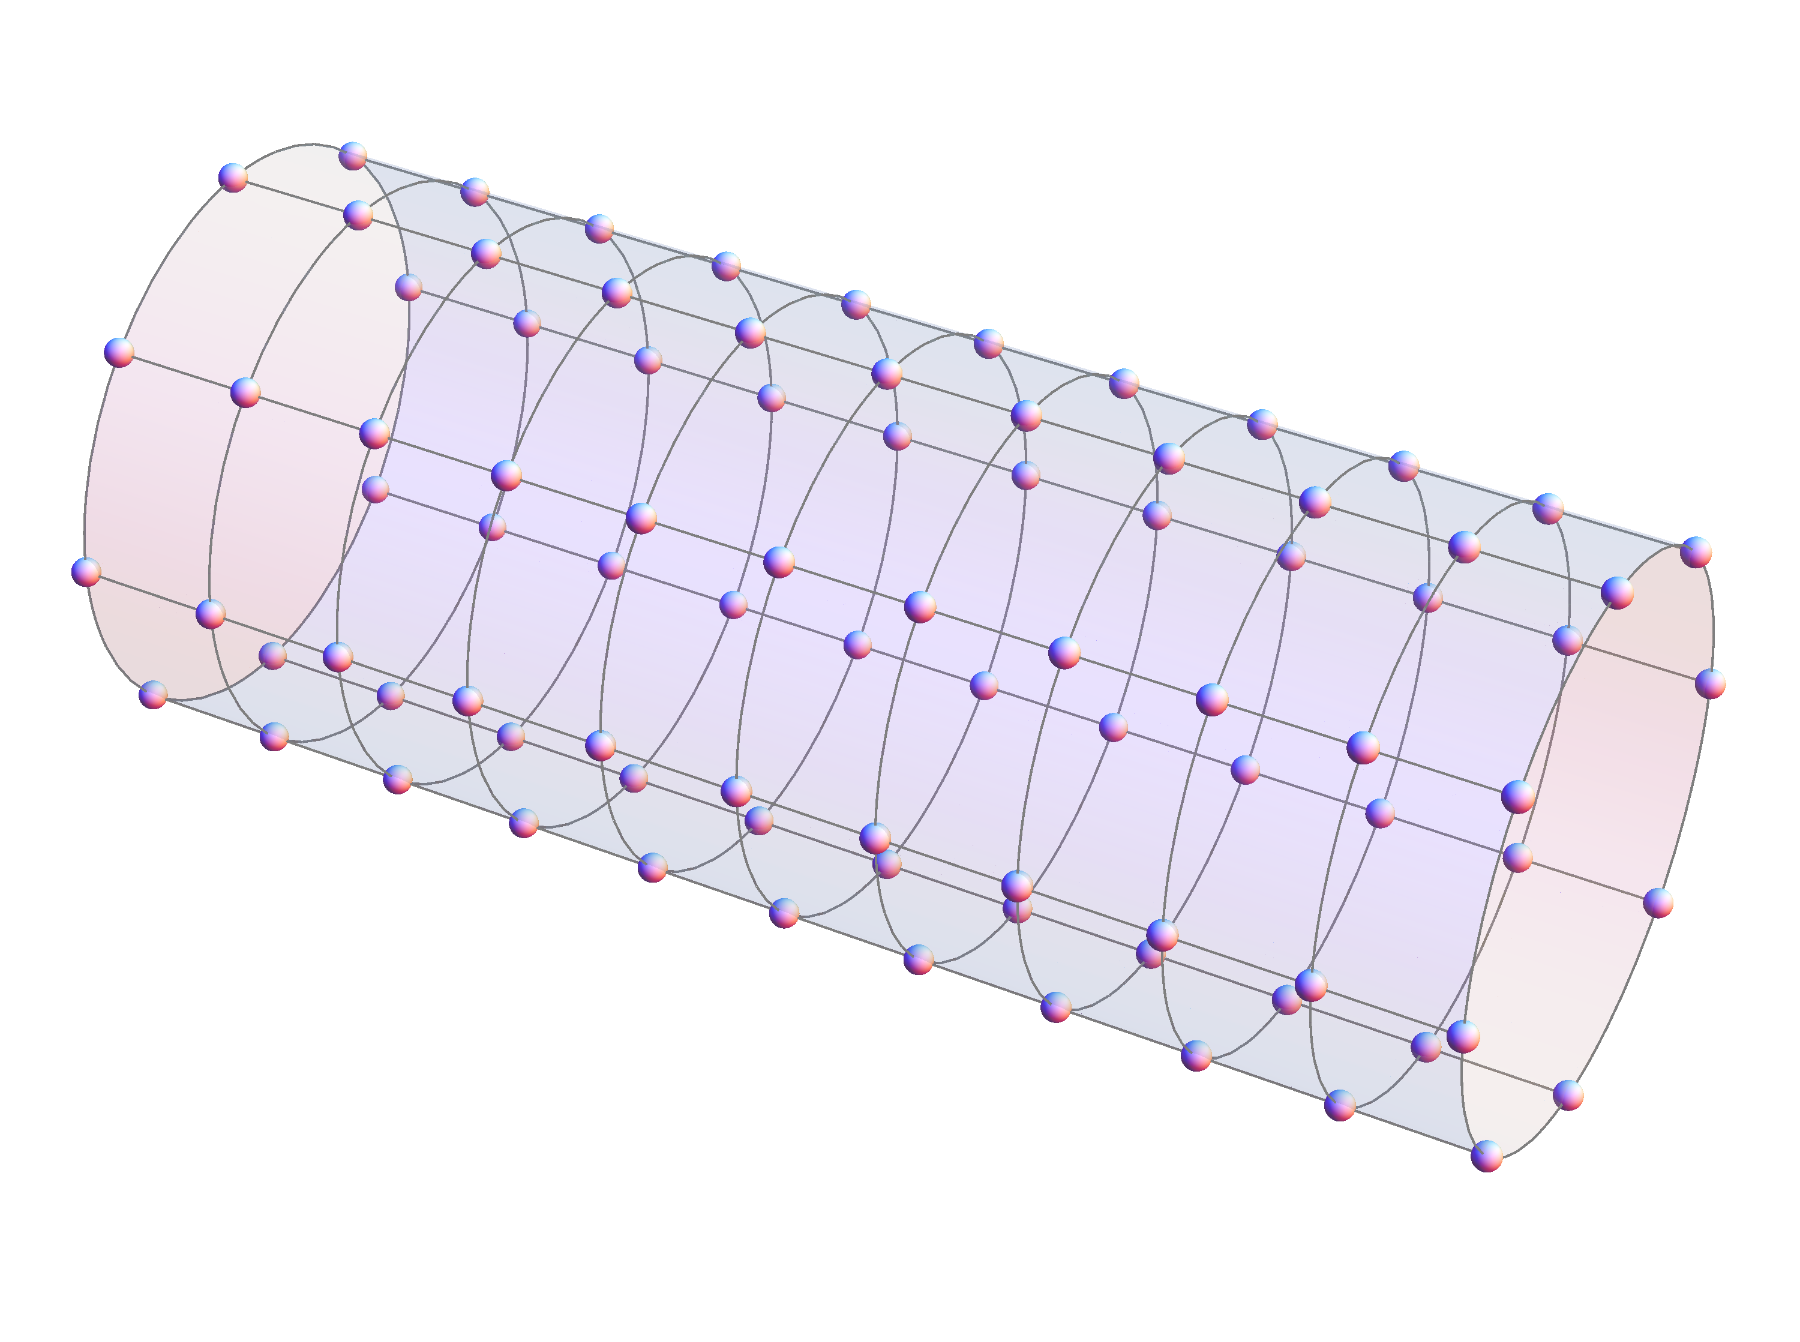
\includegraphics[scale=0.2]{Graphics/TransferMatrix/lattice_cylinder.png}
\caption{A single boundary condition in the vertical direction wraps the square lattice into a cylinder.}
\label{fig:cylinder} 
\end{figure}
%
Expanding on the two dimensional model we can consider the lattice subject to just one boundary condition, \eqref{2disingboundarycondition2}, and find an expression for the partition function when the topology of the lattice is folded into a cylinder.  We continue from \eqref{tm_torus}, but omit the final transfer matrix $T\left(\xi_C,\xi_1\right)$. The partition function becomes
%
\begin{align}
\label{tm_cylinder}
Z=\sum_{\xi_1}\sum_{\xi_2}...\sum_{\xi_C}&T\left(\xi_1,\xi_2\right)T\left(\xi_2,\xi_3\right)T\left(\xi_3,\xi_4\right)...T\left(\xi_{C-1},\xi_C\right)\\
&\times\exp\left(-\frac{\beta H\left( \xi_1\right)}{2}\right)\exp\left(-\frac{\beta H\left( \xi_C\right)}{2}\right)
\end{align}
%
Here we introduce a Kronecker delta function with a dummy variable $\xi_\alpha$ such that
%
\begin{equation}\label{bc_cylin}
\delta_{\xi_1,\xi_\alpha}=\sum_{\mu}\psi_{\mu}^{*}\left(\xi_{1} \right)\psi_{\mu}\left(\xi_{\alpha}\right)
\end{equation}
%
Inserting this into \eqref{tm_cylinder} 

%
\begin{align}
Z\left(\xi_{\alpha}\right)=\sum_{\mu}\sum_{\xi_1}\sum_{\xi_2}...\sum_{\xi_C}&\psi_{\mu}^{*}\left(\xi_{1} \right)T\left(\xi_1,\xi_2\right)T\left(\xi_2,\xi_3\right)T\left(\xi_3,\xi_4\right)...T\left(\xi_{C-1},\xi_C\right)\psi_{\mu}\left(\xi_{\alpha}\right)\\
&\times\exp\left(-\frac{\beta H\left( \xi_1\right)}{2}\right)\exp\left(-\frac{\beta H\left( \xi_C\right)}{2}\right)\nonumber
\end{align}
%
We then proceed to contract each transfer matrix in the sum from $\xi_1$ to get an expression for the partition function
%
\begin{equation}
Z\left(\xi_{\alpha}\right)=\sum_{\mu}\sum_{\xi_C}\lambda_{\mu}^{C-1}\psi_{\mu}^{*}\left(\xi_{C} \right)\psi_{\mu}\left(\xi_{\alpha}\right)\exp\left(-\frac{\beta H\left( \xi_{\alpha}\right)}{2}\right)\exp\left(-\frac{\beta H\left( \xi_C\right)}{2}\right)
\end{equation}


